\documentclass{uebblatt}

\usepackage{draftwatermark}
\definecolor{pink}{rgb}{0.95,0.9,0.95}
\SetWatermarkText{\textsf{\textcolor{pink}{ENTWURF}}}
\SetWatermarkScale{1}

\newcommand{\Ch}{\mathrm{Ch}}

\newcommand{\Cyl}{\mathrm{Cyl}}

\begin{document}

\maketitle{14}{}

\begin{aufgabe}{Ein abstrakter Zugang zum Würfellemma}
Die Aussage von Aufgabe~1b) von Blatt~11 heißt auch \emph{Würfellemma}. Führe
einen neuen Beweis dieses Lemmas, aber auf folgende Art und Weise. Mache die
Kategorie~$\B \defeq (b \leftarrow a \rightarrow c)$ zu einer Reedy-Kategorie,
in der~$a \to b$ den Grad erhöht und~$a \to c$ ihn erniedrigt. Zeige, dass dann
ein kofaserndes Objekt in der Funktorkategorie~$[\B,\C]$ bezüglich der
Reedy-Modellstruktur, wobei~$\C$ eine beliebige Modellkategorie ist, gerade ein
solches Diagramm~$(B \leftarrow A \rightarrow C)$ ist, in dem~$A$,~$B$ und~$C$ kofasernd
und~$A \to B$ eine Kofaserung ist. Zeige schließlich, dass der Funktor~$[\B,\C]
\xra{\colim} \C$ ein Links-Quillen-Funktor ist, indem du nachweist, dass sein
Rechtsadjungierter~$\C \to [\B,\C]$, der einem Objekt~$X$ das konstante
Diagramm~$(X \leftarrow X \rightarrow X)$ zuweist, schwache Äquivalenzen und
Faserungen bewahrt.
\end{aufgabe}
% Hovey 5.2.6

\begin{aufgabe}{Zylinderobjekte bei Kettenkomplexen}
Sei für ein Kettenkomplex~$V_\bullet \in \Ch_{\geq0}(R)$ sein \emph{Zylinder}
definiert als der Kettenkomplex~$\Cyl(V_\bullet)$ mit~$\Cyl(V_\bullet)_m = V_m
\oplus V_{m-1} \oplus V_m$ und Differential~$\partial(a,b,c) = (\partial a + b,
-\partial b, \partial c - b)$, zusammen mit den Komplexmorphismen~$i_0, i_1 :
V_\bullet \to \Cyl(V_\bullet)$ und~$p : \Cyl(V_\bullet) \to V_\bullet$
mit~$i_0(x) = (x,0,0)$, $i_1(x) = (0,0,x)$ und~$p(a,b,c) = a+c$.

Zeige, dass diese Konstruktion bezüglich der projektiven Modellstruktur ein
Zylinderobjekt von~$V_\bullet$ definiert. Wann ist dieses gut?
\end{aufgabe}
% http://math.stackexchange.com/questions/326471/cylinder-object-in-the-model-category-of-chain-complexes

\begin{aufgabe}{Kogruppenstruktur auf dem Einheitskreis}
Schlage die Definition einer \emph{Kogruppe} nach und beweise, dass der
Einheitskreis~$S^1$ in der Kategorie der punktierten topologischen Räume
modulo Homotopie eine interessante Kogruppenstruktur zulässt.
\end{aufgabe}

Noch zu \TeX en: Prop.~5.1.4 und Cor.~5.1.5 aus Hovey; kosimpliziale
Auflösungen in $\Ch_{\geq0}(R)$ und Berechnung von $A \otimes^L K$
für $A \in Ch_{\geq0}(R)$, $K \in \sSet$ (Tipp: Dold-Kan).

\vfill
\centering
\href{https://www.nasa.gov/mission_pages/newhorizons/images/index.html}{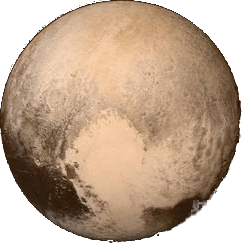
\includegraphics[scale=0.4]{images/pluto}}
\par

\end{document}

Aus dem Hovey:

1) Prop. 5.1.4
2) Cor. 5.1.5.
5) Kosimpliziale Auflösungen in Ch_*(R) und Berechnung von A \otimes^L K
für A \in Ch_*(R), K \in sSet (Tip: Dold-Kan)

Die Operation von S = Ho sSet auf Ho Ch_*(R) nochmals für S_* = Ho sSet_*
punktiert und mit dem Smash-Produkt. Was ist dann A \smash S^1?

Berechnen Sie die kanonische Faser- und Kofasersequenz für die Kategorie
der Kettenkomplexe (Siehe 6.1 und 6.2 in Hovey.)

Gruppen und Ko-Gruppenstruktur auf \Omega A und \Sigma A
